
\documentclass[11pt]{article}
\usepackage[margin=0.72in]{geometry}
\usepackage[utf8]{inputenc}
\usepackage[T1]{fontenc}
\usepackage{graphicx}
\usepackage{booktabs}
\usepackage{tabularx}
\usepackage{longtable}
\usepackage{array}
\usepackage{enumitem}
\usepackage{xcolor}
\usepackage{hyperref}
\usepackage{float}
\usepackage{tikz}
\usetikzlibrary{arrows.meta,positioning,shapes.geometric,shapes.misc,fit,calc,backgrounds}
\hypersetup{colorlinks=true, linkcolor=blue!50!black, urlcolor=blue!50!black, citecolor=blue!50!black}
\setlist[itemize]{leftmargin=*, itemsep=2pt, topsep=3pt}
\setlist[enumerate]{leftmargin=*, itemsep=2pt, topsep=3pt}
\definecolor{branddark}{HTML}{071013}
\definecolor{brandwhite}{HTML}{F9FAF6}
\definecolor{brandyellow}{HTML}{F4C542}
\definecolor{okgreen}{HTML}{2E7D32}
\definecolor{warnorange}{HTML}{EF8E23}
\definecolor{dangerred}{HTML}{C62828}
\definecolor{infoblue}{HTML}{1E88E5}
\newcolumntype{Y}{>{\raggedright\arraybackslash}X}
\newcommand{\code}[1]{\texttt{#1}}
\newcommand{\todo}[1]{\textbf{#1}}
\title{Extended Production Architecture and Backlog Expansion Plan\\\large Blockchain-Based E-Procurement and PLS Financing Seedbed}
\author{Prepared for the Blockchain-Based E-Procurement System Project}
\date{2026-05-26}
\begin{document}
\maketitle

\begin{abstract}
This document extends the current supervisor-demo-ready Digital Procurement and PLS Seedbed MVP toward a deployable and eventually production-capable model. The current repository evidence should continue to be interpreted conservatively: the application is ready for supervisor demonstration, not yet pilot-ready or commercial-ready. The proposed extension adds modular production Fabric consortium support, sandbox-swappable payment settlement, escrow release and dispute workflows, IoT/QR/EPCIS logistics proof, production document handling, Shariah certification artifacts, export signing and key management, ERP/accounting integration, ISO 20022 payment execution, richer blockchain status visualization, improved responsive UI/UX, real database-seeded demo accounts, and external APIs for IoT and integrations. The plan also expands the backlog with implementable PBIs and includes behavioral UML diagrams and extended architecture diagrams for engineering handoff.
\end{abstract}

\tableofcontents
\newpage

\section{Current Baseline and Planning Assumptions}

\subsection{Current origin/main state}
The repository has reached a supervisor-demo release-candidate baseline. The current application demonstrates authenticated actor routing, administrator governance surfaces, compliance review, buyer/supplier procurement flow, delivery evidence metadata/hash flow, escrow, blockchain proof panels, proof timeline, Shariah review, financier PLS scenario simulator, regulator export bundle, security-operator surfaces, guided demo mode, PostgreSQL dry-run validation, and Fabric chaincode build/test evidence.

\textbf{Assumption A1.} The current release-candidate evidence is accurate and corresponds to the latest origin/main. This plan does not independently re-run runtime validation. It uses the repository evidence file \code{docs/evidence/qa/FINAL\_RELEASE\_CANDIDATE\_VALIDATION.md} as current baseline.

\textbf{Assumption A2.} The next target is not immediate production operation. The next target is a deployable internal pilot model, then production hardening.

\textbf{Assumption A3.} The architecture must remain modular: payments, Fabric, IoT/logistics, ERP/accounting, and document-signature verification must be replaceable behind application ports and adapters.

\subsection{Baseline readiness statement}
The safe status remains:

\begin{quote}
Supervisor demo ready, not pilot-ready or commercial-ready.
\end{quote}

The proposed work therefore separates:

\begin{itemize}
  \item \textbf{Deployable internal pilot scope}: Dockerized app, PostgreSQL live persistence, environment configuration, operator runbooks, sandbox payment adapter, non-production key management, and controlled demo data.
  \item \textbf{Production capability scope}: production Fabric consortium, formal signing key management, external payment rails, external ERP/accounting integration, formal Shariah certification, legal retention and privacy controls.
\end{itemize}

\section{Reference Images and UI Direction}

The attached UI references imply two design requirements: an operator-grade navigation model with compact icon state, and a complete UML/architecture documentation taxonomy for future engineering communication.



\begin{figure}[H]
\centering
\resizebox{0.95\linewidth}{!}{%
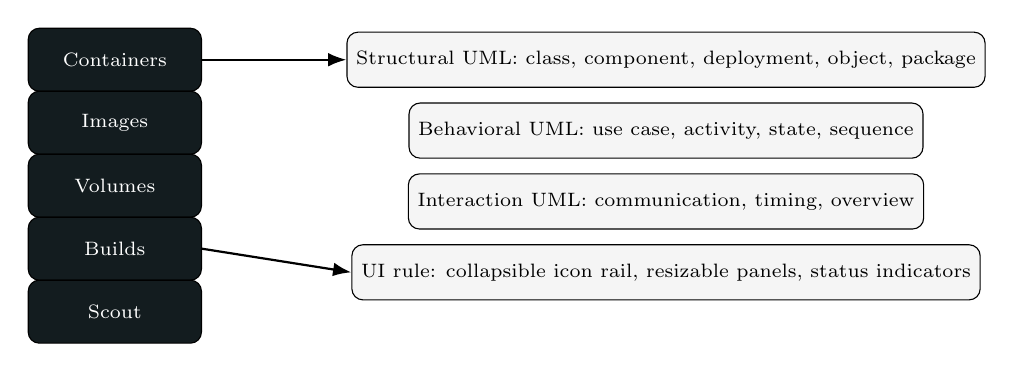
\begin{tikzpicture}[every node/.style={font=\scriptsize}, nav/.style={draw, rounded corners, align=center, fill=branddark!95, text=white, minimum width=22mm, minimum height=8mm}, item/.style={draw, rounded corners, align=left, fill=gray!8, minimum width=55mm, minimum height=7mm}]
\node[nav] (n1) at (0,0) {Containers};
\node[nav] (n2) at (0,-0.8) {Images};
\node[nav] (n3) at (0,-1.6) {Volumes};
\node[nav] (n4) at (0,-2.4) {Builds};
\node[nav] (n5) at (0,-3.2) {Scout};
\node[item] (s1) at (7,0) {Structural UML: class, component, deployment, object, package};
\node[item] (s2) at (7,-0.9) {Behavioral UML: use case, activity, state, sequence};
\node[item] (s3) at (7,-1.8) {Interaction UML: communication, timing, overview};
\node[item] (s4) at (7,-2.7) {UI rule: collapsible icon rail, resizable panels, status indicators};
\draw[-Latex, thick] (n1.east) -- (s1.west);
\draw[-Latex, thick] (n4.east) -- (s4.west);
\end{tikzpicture}%
}
\caption{Input design interpretation. The product shell should provide compact icon navigation, resizable panels, clear visual status indicators, and UML-backed architecture documentation.}
\label{fig:inputrefs}
\end{figure}



\section{Market and Standards Research Summary}

\subsection{Procurement and contracting model}
The Open Contracting Data Standard (OCDS) is relevant for public or regulated procurement transparency. OCDS describes a common data model for disclosure at multiple contracting stages and is intended to support analysis and transparency. For this system, OCDS should be used as an optional export/mapping model for tender, award, contract, implementation, and document metadata rather than replacing the operational database.

\subsection{Machine-readable business documents}
OASIS Universal Business Language (UBL), ISO/IEC 19845, is relevant for structured procurement documents such as orders, order responses, despatch advice, invoices, and related supply chain documents. The system should treat UBL as an import/export adapter format, not as the internal domain model. Peppol BIS can be considered for regional procurement document exchange profiles.

\subsection{Logistics proof and EPCIS}
GS1 EPCIS 2.0 is suitable for visibility event data across enterprises and can support object/event traceability for shipment, receipt, inspection, and logistics milestones. The proposed IoT/logistics API should generate an internal delivery evidence record first, then optionally map to EPCIS ObjectEvent, AggregationEvent, TransactionEvent, TransformationEvent, or AssociationEvent where the data is available.

\subsection{Payment standards}
ISO 20022 is the reference model for financial-industry message definitions. Payment execution should be isolated behind a payment orchestration port with pluggable sandbox adapters before any real bank integration. The first payment adapter should be an open-source or local mock/sandbox gateway that can emit ISO 20022-like payment initiation and status artifacts without moving real money.

\subsection{Fabric production architecture}
Hyperledger Fabric is appropriate for enterprise permissioned networks because participants are identifiable, networks are permissioned, and consensus, membership, and endorsement are modular. The production plan should therefore use Fabric for proof anchoring, selective private data, endorsement policy, and governance records, but not as the operational database.

\section{Extended Architecture Objectives}

\begin{enumerate}
  \item Add production Fabric consortium support while preserving local/in-memory proof modes.
  \item Introduce a swappable payment integration layer with sandbox-first implementation.
  \item Extend escrow from creation-only to release, hold, dispute, arbitration, and settlement instruction workflows.
  \item Add IoT/QR/EPCIS/logistics proof ingestion APIs with signed evidence metadata.
  \item Add production-grade document upload, preview, rendering, malware scanning, and signature verification.
  \item Add formal Shariah certification workflow and versioned certificate artifacts.
  \item Add export signing, key management, and offline verification tools.
  \item Add ERP/accounting adapter framework and machine-readable procurement/contract mappings.
  \item Improve UI/UX with resizable panels, icon-only collapsed state, visual indicators, dark/white/yellow theme, and overflow-resilient containers.
  \item Replace demonstrative/local fallback paths with real demo accounts seeded into the database.
\end{enumerate}

\section{Modular Target Architecture}



\begin{figure}[H]
\centering
\resizebox{\linewidth}{!}{%
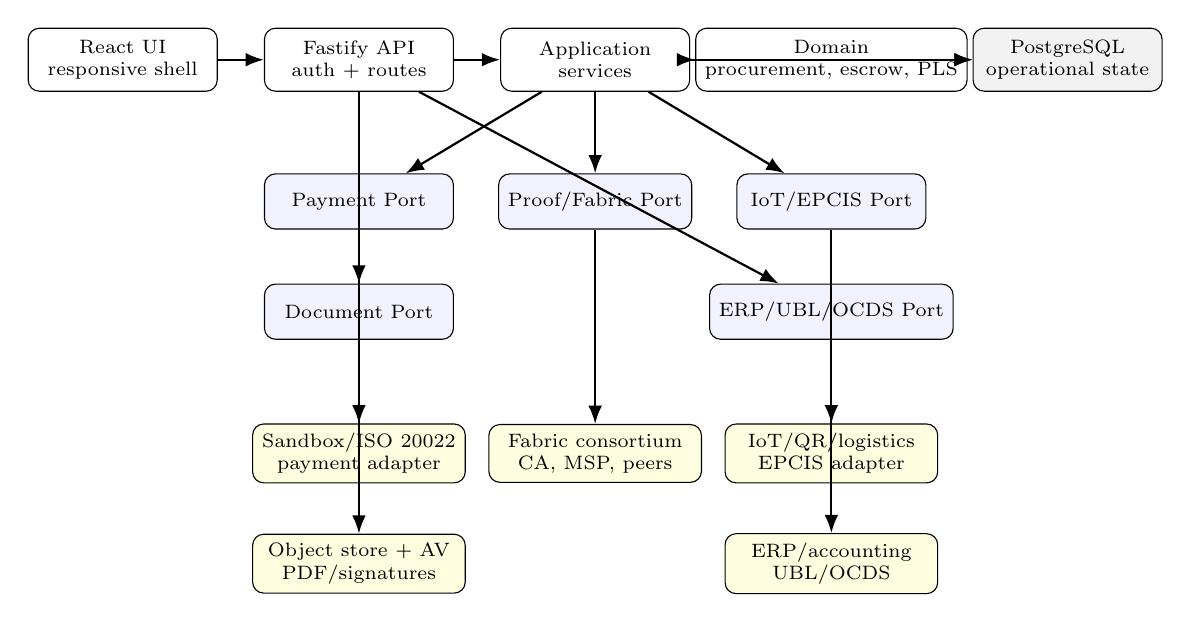
\begin{tikzpicture}[every node/.style={font=\scriptsize}, box/.style={draw, rounded corners, align=center, minimum width=24mm, minimum height=8mm, fill=white}, port/.style={draw, rounded corners, align=center, minimum width=24mm, minimum height=7mm, fill=blue!5}, ext/.style={draw, rounded corners, align=center, minimum width=27mm, minimum height=7mm, fill=yellow!12}, arr/.style={-Latex, thick}]
\node[box] (ui) at (0,0) {React UI\\responsive shell};
\node[box] (api) at (3,0) {Fastify API\\auth + routes};
\node[box] (app) at (6,0) {Application\\services};
\node[box] (domain) at (9,0) {Domain\\procurement, escrow, PLS};
\node[box, fill=gray!10] (db) at (12,0) {PostgreSQL\\operational state};
\node[port] (payport) at (3,-1.8) {Payment Port};
\node[port] (fabricport) at (6,-1.8) {Proof/Fabric Port};
\node[port] (iotport) at (9,-1.8) {IoT/EPCIS Port};
\node[port] (docport) at (3,-3.2) {Document Port};
\node[port] (erpport) at (9,-3.2) {ERP/UBL/OCDS Port};
\node[ext] (pay) at (3,-5) {Sandbox/ISO 20022\\payment adapter};
\node[ext] (fabric) at (6,-5) {Fabric consortium\\CA, MSP, peers};
\node[ext] (iot) at (9,-5) {IoT/QR/logistics\\EPCIS adapter};
\node[ext] (doc) at (3,-6.4) {Object store + AV\\PDF/signatures};
\node[ext] (erp) at (9,-6.4) {ERP/accounting\\UBL/OCDS};
\draw[arr] (ui) -- (api); \draw[arr] (api) -- (app); \draw[arr] (app) -- (domain); \draw[arr] (domain) -- (db); \draw[arr] (app) -- (db);
\draw[arr] (app) -- (payport); \draw[arr] (app) -- (fabricport); \draw[arr] (app) -- (iotport); \draw[arr] (api) -- (docport); \draw[arr] (api) -- (erpport);
\draw[arr] (payport) -- (pay); \draw[arr] (fabricport) -- (fabric); \draw[arr] (iotport) -- (iot); \draw[arr] (docport) -- (doc); \draw[arr] (erpport) -- (erp);
\end{tikzpicture}%
}
\caption{Extended modular architecture. Production services are plugged into ports/adapters so sandbox payment, local Fabric, external Fabric, IoT/EPCIS, and ERP connectors can be swapped without contaminating domain logic.}
\label{fig:component}
\end{figure}



\subsection{Core modular rules}
\begin{itemize}
  \item Domain/application layers must not import payment SDKs, Fabric SDKs, ERP SDKs, IoT SDKs, object-storage clients, or PDF rendering libraries.
  \item External systems communicate through explicit ports and adapters.
  \item PostgreSQL remains the system of record for operational workflow state.
  \item Fabric stores proof, endorsement, governance, and selected private-data hashes; raw business documents remain off-chain.
  \item Payment settlement is an instruction and reconciliation workflow until real rails are certified.
\end{itemize}

\section{Deployment Architecture}

\begin{figure}[H]
\centering
\resizebox{\linewidth}{!}{%
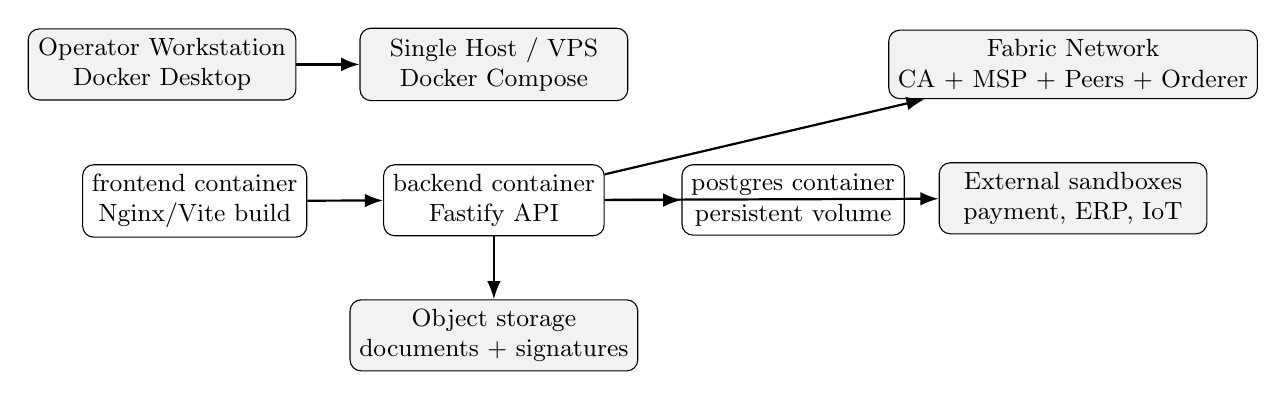
\begin{tikzpicture}[node distance=8mm and 8mm, every node/.style={font=\small}, nodebox/.style={draw, rounded corners, align=center, minimum width=28mm, minimum height=8mm, fill=white}, infra/.style={draw, rounded corners, align=center, fill=gray!10, minimum width=34mm, minimum height=8mm}, arr/.style={-Latex, thick}]
\node[infra] (operator) {Operator Workstation\\Docker Desktop};
\node[infra, right=of operator] (host) {Single Host / VPS\\Docker Compose};
\node[nodebox, below=of host, xshift=-38mm] (frontend) {frontend container\\Nginx/Vite build};
\node[nodebox, below=of host] (backend) {backend container\\Fastify API};
\node[nodebox, below=of host, xshift=38mm] (postgres) {postgres container\\persistent volume};
\node[infra, right=of host, xshift=25mm] (fabric) {Fabric Network\\CA + MSP + Peers + Orderer};
\node[infra, below=of fabric] (external) {External sandboxes\\payment, ERP, IoT};
\node[infra, below=of backend] (object) {Object storage\\documents + signatures};
\draw[arr] (operator) -- (host);
\draw[arr] (frontend) -- (backend);
\draw[arr] (backend) -- (postgres);
\draw[arr] (backend) -- (fabric);
\draw[arr] (backend) -- (external);
\draw[arr] (backend) -- (object);
\end{tikzpicture}%
}
\caption{Deployable internal pilot deployment model. The first deployable model should target single-host Docker Compose with optional external Fabric and sandbox integrations.}
\label{fig:deployment}
\end{figure}

\section{Behavioral UML Diagrams}

\subsection{Use Case Diagram}



\begin{figure}[H]
\centering
\resizebox{\linewidth}{!}{%
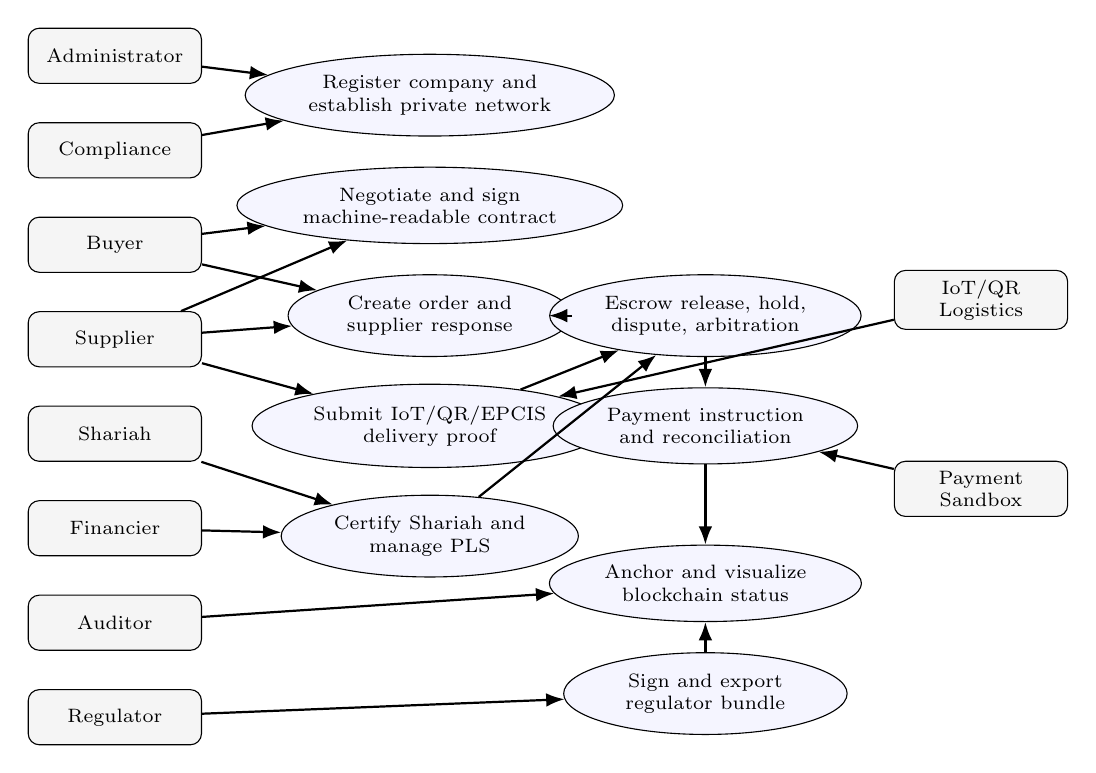
\begin{tikzpicture}[every node/.style={font=\scriptsize}, actor/.style={draw, rounded corners, align=center, minimum width=22mm, minimum height=7mm, fill=gray!8}, uc/.style={draw, ellipse, align=center, minimum width=36mm, minimum height=8mm, fill=blue!4}, arr/.style={-Latex, thick}]
\node[actor] (admin) at (0,3.5) {Administrator};
\node[actor] (comp) at (0,2.3) {Compliance};
\node[actor] (buyer) at (0,1.1) {Buyer};
\node[actor] (supp) at (0,-0.1) {Supplier};
\node[actor] (shar) at (0,-1.3) {Shariah};
\node[actor] (fin) at (0,-2.5) {Financier};
\node[actor] (aud) at (0,-3.7) {Auditor};
\node[actor] (regu) at (0,-4.9) {Regulator};
\node[actor] (iotact) at (11,0.4) {IoT/QR\\Logistics};
\node[actor] (payact) at (11,-2.0) {Payment\\Sandbox};
\node[uc] (registration) at (4,3.0) {Register company and\\establish private network};
\node[uc] (contract) at (4,1.6) {Negotiate and sign\\machine-readable contract};
\node[uc] (order) at (4,0.2) {Create order and\\supplier response};
\node[uc] (delivery) at (4,-1.2) {Submit IoT/QR/EPCIS\\delivery proof};
\node[uc] (escrow) at (7.5,0.2) {Escrow release, hold,\\dispute, arbitration};
\node[uc] (payment) at (7.5,-1.2) {Payment instruction\\and reconciliation};
\node[uc] (pls) at (4,-2.6) {Certify Shariah and\\manage PLS};
\node[uc] (proof) at (7.5,-3.2) {Anchor and visualize\\blockchain status};
\node[uc] (export) at (7.5,-4.6) {Sign and export\\regulator bundle};
\draw[arr] (admin) -- (registration); \draw[arr] (comp) -- (registration);
\draw[arr] (buyer) -- (contract); \draw[arr] (supp) -- (contract); \draw[arr] (buyer) -- (order); \draw[arr] (supp) -- (order); \draw[arr] (supp) -- (delivery); \draw[arr] (iotact) -- (delivery);
\draw[arr] (order) -- (escrow); \draw[arr] (delivery) -- (escrow); \draw[arr] (escrow) -- (payment); \draw[arr] (payact) -- (payment);
\draw[arr] (shar) -- (pls); \draw[arr] (fin) -- (pls); \draw[arr] (pls) -- (escrow); \draw[arr] (payment) -- (proof); \draw[arr] (aud) -- (proof); \draw[arr] (regu) -- (export); \draw[arr] (export) -- (proof);
\end{tikzpicture}%
}
\caption{Extended use case diagram. New production work connects company registration, private network establishment, negotiation, delivery proof, escrow release/dispute, payment settlement, blockchain visualization, and signed exports.}
\label{fig:usecase}
\end{figure}



\subsection{Activity Diagram: Company to Settlement}

\begin{figure}[H]
\centering
\resizebox{0.95\linewidth}{!}{%
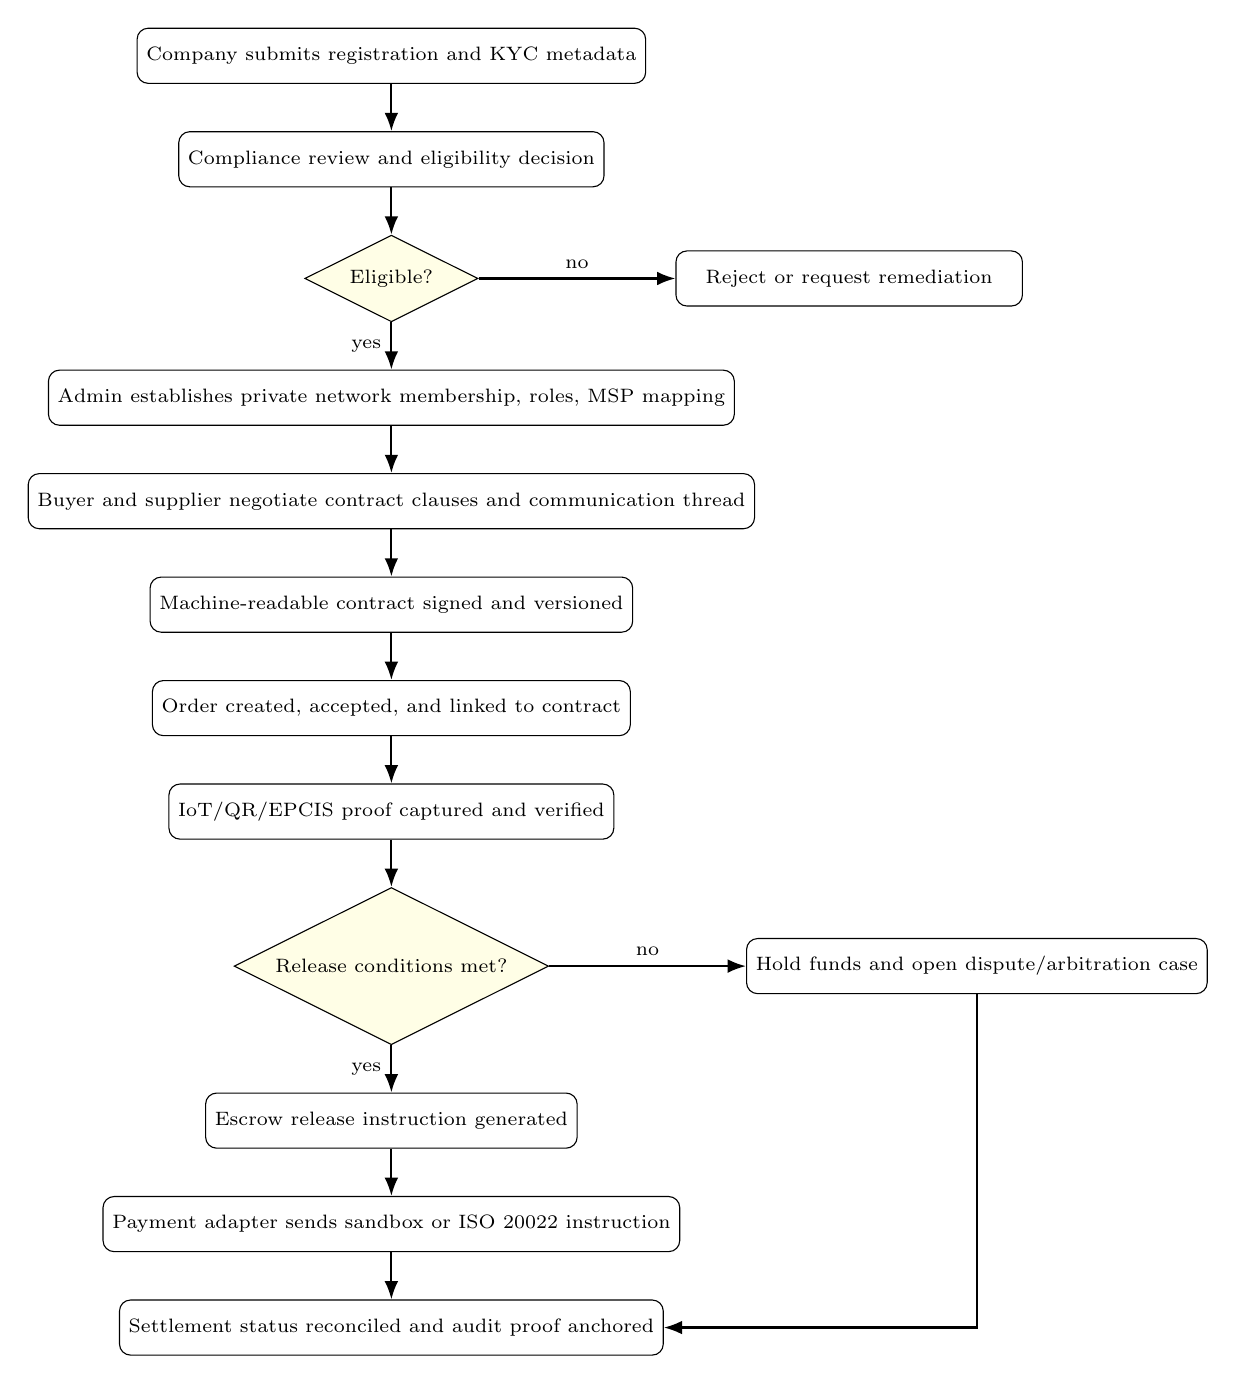
\begin{tikzpicture}[node distance=6mm, every node/.style={font=\scriptsize}, actstep/.style={draw, rounded corners, align=center, fill=white, minimum width=44mm, minimum height=7mm}, decision/.style={draw, diamond, aspect=2, align=center, fill=yellow!10}, arr/.style={-Latex, thick}]
\node[actstep] (start) {Company submits registration and KYC metadata};
\node[actstep, below=of start] (kyc) {Compliance review and eligibility decision};
\node[decision, below=of kyc] (eligible) {Eligible?};
\node[actstep, below=of eligible] (network) {Admin establishes private network membership, roles, MSP mapping};
\node[actstep, below=of network] (negotiate) {Buyer and supplier negotiate contract clauses and communication thread};
\node[actstep, below=of negotiate] (sign) {Machine-readable contract signed and versioned};
\node[actstep, below=of sign] (order) {Order created, accepted, and linked to contract};
\node[actstep, below=of order] (delivery) {IoT/QR/EPCIS proof captured and verified};
\node[decision, below=of delivery] (releaseok) {Release conditions met?};
\node[actstep, below=of releaseok] (release) {Escrow release instruction generated};
\node[actstep, below=of release] (payment) {Payment adapter sends sandbox or ISO 20022 instruction};
\node[actstep, below=of payment] (recon) {Settlement status reconciled and audit proof anchored};
\node[actstep, right=25mm of eligible] (reject) {Reject or request remediation};
\node[actstep, right=25mm of releaseok] (dispute) {Hold funds and open dispute/arbitration case};
\draw[arr] (start) -- (kyc); \draw[arr] (kyc) -- (eligible); \draw[arr] (eligible) -- node[left]{yes} (network); \draw[arr] (eligible) -- node[above]{no} (reject); \draw[arr] (network) -- (negotiate); \draw[arr] (negotiate) -- (sign); \draw[arr] (sign) -- (order); \draw[arr] (order) -- (delivery); \draw[arr] (delivery) -- (releaseok); \draw[arr] (releaseok) -- node[left]{yes} (release); \draw[arr] (releaseok) -- node[above]{no} (dispute); \draw[arr] (release) -- (payment); \draw[arr] (payment) -- (recon); \draw[arr] (dispute) |- (recon);
\end{tikzpicture}%
}
\caption{Behavioral activity diagram for the extended production workflow.}
\label{fig:activity}
\end{figure}

\subsection{Sequence Diagram: Escrow Release and Payment Adapter}

\begin{figure}[H]
\centering
\resizebox{\linewidth}{!}{%
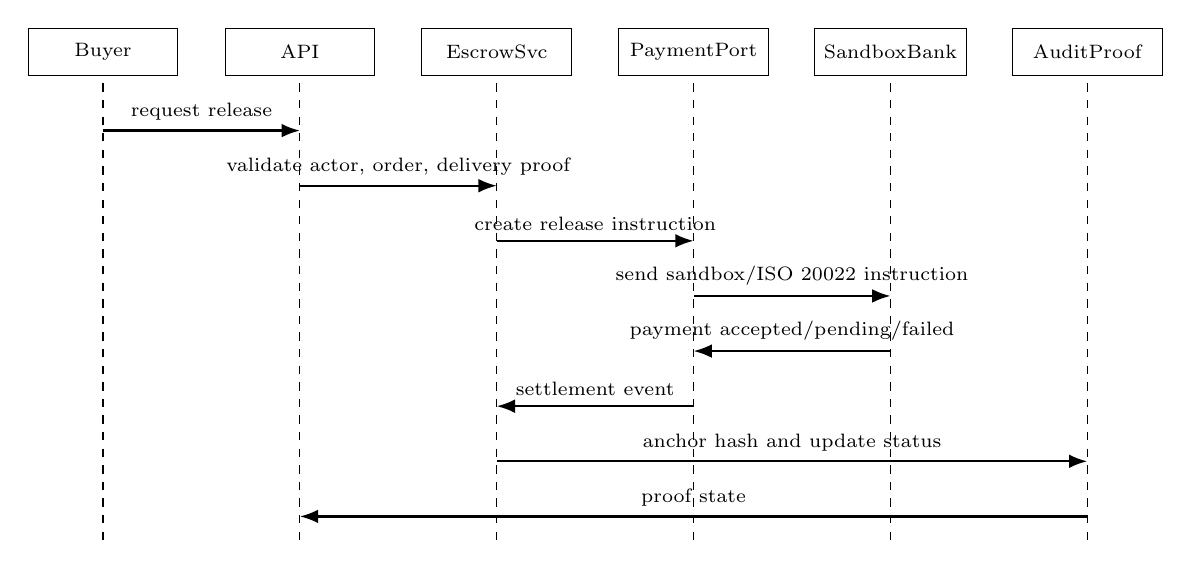
\begin{tikzpicture}[every node/.style={font=\scriptsize}, lifeline/.style={draw, minimum width=19mm, minimum height=6mm, fill=white}, arr/.style={-Latex, thick}]
\foreach \x/\name in {0/Buyer,2.5/API,5/EscrowSvc,7.5/PaymentPort,10/SandboxBank,12.5/AuditProof} {\node[lifeline] (n\x) at (\x,0) {\name}; \draw[dashed] (\x,-0.4) -- (\x,-6.2);}
\draw[arr] (0,-1) -- node[above]{request release} (2.5,-1);
\draw[arr] (2.5,-1.7) -- node[above]{validate actor, order, delivery proof} (5,-1.7);
\draw[arr] (5,-2.4) -- node[above]{create release instruction} (7.5,-2.4);
\draw[arr] (7.5,-3.1) -- node[above]{send sandbox/ISO 20022 instruction} (10,-3.1);
\draw[arr] (10,-3.8) -- node[above]{payment accepted/pending/failed} (7.5,-3.8);
\draw[arr] (7.5,-4.5) -- node[above]{settlement event} (5,-4.5);
\draw[arr] (5,-5.2) -- node[above]{anchor hash and update status} (12.5,-5.2);
\draw[arr] (12.5,-5.9) -- node[above]{proof state} (2.5,-5.9);
\end{tikzpicture}%
}
\caption{Sequence diagram showing that real settlement is behind a swappable payment port. The first implementation should use sandbox payment and ISO 20022-like messages.}
\label{fig:sequence}
\end{figure}

\subsection{State Machine: Escrow and Dispute Lifecycle}

\begin{figure}[H]
\centering
\resizebox{\linewidth}{!}{%
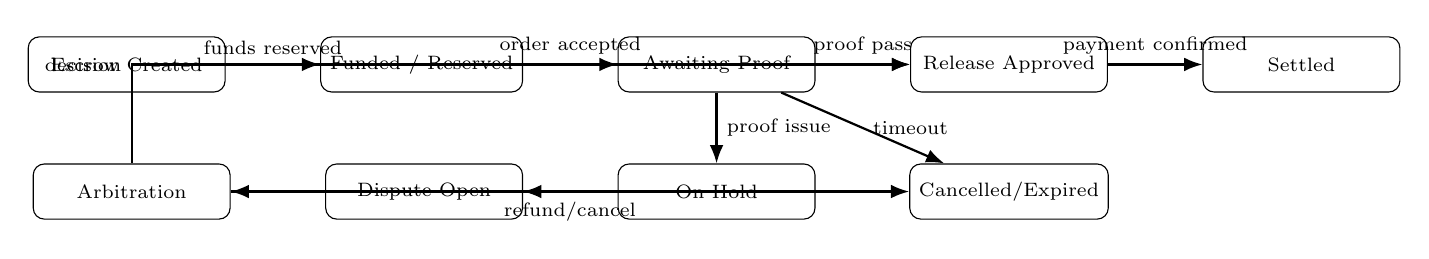
\begin{tikzpicture}[node distance=9mm and 12mm, every node/.style={font=\scriptsize}, state/.style={draw, rounded corners, align=center, minimum width=25mm, minimum height=7mm, fill=white}, arr/.style={-Latex, thick}]
\node[state] (created) {Escrow Created};
\node[state, right=of created] (funded) {Funded / Reserved};
\node[state, right=of funded] (conditions) {Awaiting Proof};
\node[state, below=of conditions] (hold) {On Hold};
\node[state, left=of hold] (dispute) {Dispute Open};
\node[state, left=of dispute] (arbitration) {Arbitration};
\node[state, right=of conditions] (release) {Release Approved};
\node[state, right=of release] (settled) {Settled};
\node[state, below=of release] (cancelled) {Cancelled/Expired};
\draw[arr] (created) -- node[above]{funds reserved} (funded);
\draw[arr] (funded) -- node[above]{order accepted} (conditions);
\draw[arr] (conditions) -- node[above]{proof pass} (release);
\draw[arr] (release) -- node[above]{payment confirmed} (settled);
\draw[arr] (conditions) -- node[right]{proof issue} (hold);
\draw[arr] (hold) -- (dispute);
\draw[arr] (dispute) -- (arbitration);
\draw[arr] (arbitration) |- node[left]{decision} (release);
\draw[arr] (arbitration) -- node[below]{refund/cancel} (cancelled);
\draw[arr] (conditions) -- node[right]{timeout} (cancelled);
\end{tikzpicture}%
}
\caption{State machine for the extended escrow model. The current MVP only covers the early creation/proof slice; release, dispute, and settlement require new implementation.}
\label{fig:state}
\end{figure}

\section{Production Capability Plans}

\subsection{Production Fabric consortium}
\textbf{Goal.} Move from local AuditAnchor proof toward a governed Fabric consortium with CA/MSP, organization membership, endorsement policies, private data collections, chaincode lifecycle, channel governance, and operational observability.

\textbf{Plan.}
\begin{enumerate}
  \item Define consortium members: platform operator, buyer organization, supplier organization, financier, regulator/auditor node.
  \item Add a Fabric governance registry mapping platform member organizations to MSP IDs, certificates, channel memberships, and endorsement responsibilities.
  \item Split chaincode into modules: AuditAnchor, EscrowGovernance, ExportProof, PLSCertificateProof.
  \item Use private data collections for sensitive hashes/terms where necessary; never store raw commercial documents on-chain.
  \item Add channel policy: anchor proof channel, regulator evidence channel, optional PLS governance channel.
  \item Add operations runbooks: certificate rotation, peer join, chaincode upgrade, ledger backup, disaster recovery.
\end{enumerate}

\subsection{Real payment settlement with sandbox-swappable adapter}
\textbf{Goal.} Support payment execution without hard-coding any bank or payment provider.

\textbf{Design.} Add a \code{PaymentGatewayPort} and adapters:
\begin{itemize}
  \item \code{LocalSandboxPaymentAdapter}: deterministic mock for tests and demos.
  \item \code{ISO20022FileAdapter}: emits pain.001-like payment initiation artifacts and consumes status reports.
  \item \code{OpenSourceGatewayAdapter}: pluggable adapter for any selected open-source payment sandbox after evaluation.
  \item \code{ManualSettlementAdapter}: operator-reviewed fallback for regulated demos.
\end{itemize}

\textbf{Contract.} Payment state should be \code{draft}, \code{submitted}, \code{accepted}, \code{pendingSettlement}, \code{settled}, \code{failed}, \code{returned}, or \code{cancelled}. Escrow release must create a payment instruction, not directly mutate settlement state without confirmation.

\subsection{Escrow release, arbitration, and dispute workflow}
Add release-condition evaluation, manual hold, dispute creation, evidence exchange, arbitration decision, release or refund instruction, and audit/proof anchoring. Keep external payment execution behind the payment port.

\subsection{IoT/QR/EPCIS/logistics delivery proof}
Add an external device/API ingestion layer:
\begin{itemize}
  \item \code{POST /api/v1/external/iot/events}
  \item \code{POST /api/v1/external/qr/proofs}
  \item \code{POST /api/v1/external/epcis/events}
\end{itemize}
Requests must use device credentials, HMAC or mTLS, replay protection, schema validation, and signature verification. Accepted events become delivery evidence records and may map to EPCIS visibility events.

\subsection{Document upload, rendering, and signature verification}
Add object storage and document metadata, malware scanning, MIME validation, PDF/image preview, checksum, digital-signature validation, certificate chain metadata, and permissioned access. Raw documents must be off-chain; only hashes and signature verification summaries can be anchored.

\subsection{Formal Shariah certification}
Add a certificate artifact model: \code{certificateId}, \code{scope}, \code{contractTemplateVersion}, \code{reviewBoard}, \code{fatwaReference}, \code{issuedAt}, \code{expiresAt}, \code{conditions}, \code{revocationStatus}, and \code{certificateHash}. A PLS contract can activate only if its template version and parameters are covered by an active certificate or approved exception.

\subsection{Export signing and key management}
Add key management, signing profiles, signature algorithms, key rotation, revocation, offline verifier, signed manifest, detached signature, and regulator verification package. For MVP pilot, a local software key can be used. Production requires HSM/KMS decision.

\subsection{ERP/accounting integration}
Add an adapter framework with canonical internal payloads, mapping profiles, inbound validation, outbound transformation, idempotency keys, and reconciliation records. UBL/OCDS mappings should be export/import adapters, not the internal source of truth.

\section{Machine-Readable Contract Model}

\subsection{Essential contract fields}
A research-grade machine-readable contract should include:
\begin{itemize}
  \item parties, legal identities, addresses, registration numbers, and platform organization IDs;
  \item contract type, version, governing law, jurisdiction, language, and effective dates;
  \item goods/services lines, quantities, units, delivery location, incoterms or delivery terms;
  \item price, currency, tax, payment terms, escrow terms, release conditions, penalties;
  \item PLS terms: capital contribution, ratio, loss allocation, eligible cost definitions;
  \item obligations, acceptance criteria, delivery evidence requirements, inspection windows;
  \item dispute resolution, arbitration forum, escalation timeline, force majeure;
  \item document attachments, signature records, certificate references, audit/proof references;
  \item machine-readable clause IDs and human-readable text;
  \item status, amendment history, and hash references.
\end{itemize}

\subsection{Document standards mapping}
\begin{itemize}
  \item \textbf{UBL}: Purchase Order, Order Response, Despatch Advice, Invoice, Credit Note, Remittance Advice mapping.
  \item \textbf{OCDS}: planning, tender, award, contract, implementation, amendment, document and milestone mapping.
  \item \textbf{ISO 20022}: payment initiation and status mapping behind payment adapter.
  \item \textbf{EPCIS}: logistics visibility event mapping for proof of delivery and transport milestones.
\end{itemize}

\section{UI/UX Redesign Plan}

\subsection{Visual direction}
Adopt a dark/white/yellow theme:
\begin{itemize}
  \item dark shell: \code{\#071013};
  \item clean surfaces: \code{\#F9FAF6};
  \item primary accent: \code{\#F4C542};
  \item indicator colors: green for verified, orange for pending/warning, red for failed/mismatch, blue for informational.
\end{itemize}

\subsection{Resizable and icon-only panels}
Create a unified shell:
\begin{itemize}
  \item left navigation can be expanded, collapsed, or icon-only;
  \item content panels are resizable with minimum widths and overflow guards;
  \item cards can compress to icon+status mode when width falls below threshold;
  \item proof widgets can collapse to icon chips and expand on click;
  \item panel state is persisted per user in local profile/preferences.
\end{itemize}

\subsection{CSS architecture}
Move toward one CSS design system:
\begin{itemize}
  \item \code{src/frontend/styles/tokens.css}: colors, spacing, typography, shadows, breakpoints;
  \item \code{src/frontend/styles/layout.css}: shell, sidebar, resizable panels, grid;
  \item \code{src/frontend/styles/components.css}: buttons, cards, chips, tables, proof indicators;
  \item \code{src/frontend/styles/pages/*.css}: page-specific overrides only;
  \item no inline styles except dynamic CSS variables or measured dimensions.
\end{itemize}

\subsection{Overflow and resizing rules}
All components must define:
\begin{itemize}
  \item \code{min-width: 0} for flex children;
  \item \code{overflow-wrap: anywhere} for hashes, IDs, references;
  \item \code{text-overflow: ellipsis} for compact cards;
  \item \code{container-type: inline-size} where component sizing is needed;
  \item icon-only mode at narrow widths.
\end{itemize}

\section{External API Plan}

\subsection{API groups}
\begin{longtable}{p{0.27\linewidth}p{0.31\linewidth}p{0.32\linewidth}}
\toprule
API group & Example endpoints & Purpose \\
\midrule
IoT device ingestion & \code{/api/v1/external/iot/events} & Capture sensor, temperature, location, custody events. \\
QR evidence & \code{/api/v1/external/qr/proofs} & Capture signed QR proof or handover scan. \\
EPCIS ingestion & \code{/api/v1/external/epcis/events} & Accept EPCIS-compatible logistics visibility events. \\
ERP adapter & \code{/api/v1/integrations/erp/orders} & Import/export orders, invoices, receipts. \\
Payment adapter & \code{/api/v1/payments/instructions} & Create settlement instructions and status callbacks. \\
Export verifier & \code{/api/v1/exports/:id/verify} & Verify signed bundle and proof metadata. \\
\bottomrule
\end{longtable}

\subsection{Security requirements}
External APIs require API clients, scoped credentials, mTLS or HMAC signature, idempotency keys, replay windows, rate limits, payload schema validation, audit capture, and clear separation between device identity and human actor identity.

\section{Backlog Expansion Summary}

A backlog extension CSV was created as \code{backlog/production-extension-roadmap.csv}. It uses the canonical backlog columns and starts at \code{PBI-436}. The rows are planned work for future implementation; they do not claim current completion.

\begin{longtable}{p{0.09\linewidth}p{0.25\linewidth}p{0.38\linewidth}p{0.16\linewidth}}
\toprule
PBI & Title & Main purpose & Priority \\
\midrule
PBI-436 & Production extension architecture & Parent epic for production capability plan. & P0 \\
PBI-437 & Production Fabric consortium plan & CA/MSP, channel, endorsement, node governance. & P0 \\
PBI-438 & Fabric consortium implementation & Multi-org network and chaincode lifecycle. & P1 \\
PBI-439 & Payment adapter framework & Sandbox-swappable payment port. & P0 \\
PBI-440 & ISO 20022 payment execution mapping & Payment initiation/status messages. & P1 \\
PBI-441 & Escrow release workflow & Release conditions and payment instruction. & P0 \\
PBI-442 & Dispute and arbitration workflow & Hold, dispute, arbitration, decision. & P1 \\
PBI-443 & IoT and QR evidence API & Signed external evidence ingestion. & P0 \\
PBI-444 & EPCIS logistics adapter & EPCIS-compatible visibility event mapping. & P1 \\
PBI-445 & Document storage and rendering & Upload, scan, preview, access policy. & P0 \\
PBI-446 & Signature verification & Document signature and certificate validation. & P1 \\
PBI-447 & Shariah certification artifacts & Certificate scope, versioning, revocation. & P0 \\
PBI-448 & Export signing and key management & Signed manifests and verification. & P0 \\
PBI-449 & ERP/accounting adapter framework & UBL/OCDS mapping and idempotent sync. & P1 \\
PBI-450 & Contract negotiation workspace & Communication, redlines, approvals. & P0 \\
PBI-451 & Machine-readable contract model & Clause IDs, semantics, hashes, lifecycle. & P0 \\
PBI-452 & Blockchain status visualization & Operator and actor proof dashboards. & P0 \\
PBI-453 & Responsive panel shell & Resizable and icon-only UI panels. & P0 \\
PBI-454 & Theme and design tokens & Dark/white/yellow UI system. & P1 \\
PBI-455 & CSS modularization and overflow hardening & Unified CSS and responsive text behavior. & P0 \\
PBI-456 & Database-seeded demo accounts & Remove local-only demo account dependence. & P0 \\
PBI-457 & Remove demonstrative fallbacks & Replace fake/local-only flows with real seeded data. & P0 \\
PBI-458 & External API gateway & Authenticated IoT/ERP/payment integration boundary. & P0 \\
PBI-459 & Containerized deployable model & Backend/frontend/postgres compose stack. & P0 \\
PBI-460 & Observability and incident hooks & Metrics, logs, alerts, runbooks. & P1 \\
PBI-461 & Backup/restore/rollback & Operational recovery procedures. & P1 \\
PBI-462 & Procurement research and public contracts mapping & OCDS/UBL/Peppol based process research. & P1 \\
\bottomrule
\end{longtable}

\section{Implementation Waves}

\subsection{Wave A: Deployable foundation}
\begin{itemize}
  \item PBI-456, PBI-457, PBI-459, PBI-461.
  \item Outcome: real seeded accounts, reduced demo fallbacks, full Docker Compose app stack, backup/restore runbooks.
\end{itemize}

\subsection{Wave B: UI/UX productization}
\begin{itemize}
  \item PBI-452, PBI-453, PBI-454, PBI-455.
  \item Outcome: status visualization, icon-only collapsible navigation, resizable panels, dark/white/yellow theme, overflow-safe components.
\end{itemize}

\subsection{Wave C: Contracting and negotiation}
\begin{itemize}
  \item PBI-450, PBI-451, PBI-462.
  \item Outcome: company registration, private network establishment, negotiation, communication, and machine-readable contract foundation.
\end{itemize}

\subsection{Wave D: Delivery proof and documents}
\begin{itemize}
  \item PBI-443, PBI-444, PBI-445, PBI-446.
  \item Outcome: external device/API ingestion, QR proof, EPCIS mapping, document storage/rendering/signature verification.
\end{itemize}

\subsection{Wave E: Escrow and payment}
\begin{itemize}
  \item PBI-439, PBI-440, PBI-441, PBI-442.
  \item Outcome: sandbox payment adapter, ISO 20022 mapping, release workflow, dispute/arbitration.
\end{itemize}

\subsection{Wave F: Fabric and regulated evidence}
\begin{itemize}
  \item PBI-437, PBI-438, PBI-448.
  \item Outcome: production Fabric consortium architecture, signed export packages, proper key management model.
\end{itemize}

\subsection{Wave G: Shariah and pilot readiness}
\begin{itemize}
  \item PBI-447 plus compliance/legal review PBIs from existing backlog.
  \item Outcome: formal Shariah certificate artifacts and pilot-ready governance pack.
\end{itemize}

\section{Definition of Done for Extended Work}

\begin{itemize}
  \item Code compiles and tests pass.
  \item Backlog row has evidence, acceptance criteria, and source references.
  \item All external integrations have sandbox mode and failure-state handling.
  \item UI remains responsive, accessible, and free of implementation labels.
  \item Proof and payment states are honest; no fake settlement, Fabric, or signing data.
  \item Sensitive documents and KYC data are access-controlled and never written raw on-chain.
  \item Deployment runbook and rollback guidance are updated.
\end{itemize}

\section{Immediate Next Codex Prompt}

The next implementation agent should start with Wave A and Wave B, not with production Fabric. Recommended first prompt:

\begin{quote}
Implement PBI-456 and PBI-457: seed real demo accounts and remove demonstrative local fallbacks where backend seeded data exists. Then implement PBI-453 and PBI-455 to introduce resizable, icon-only panel behavior and overflow-safe CSS architecture. Do not implement payment, Fabric consortium, IoT, or ERP until the product shell and seeded data model are stable.
\end{quote}

\begin{thebibliography}{9}
\bibitem{uml} Object Management Group, ``Unified Modeling Language 2.5.1,'' 2017. Available: \url{https://www.omg.org/spec/UML/2.5.1/}
\bibitem{fabric} Hyperledger Foundation, ``Hyperledger Fabric Introduction,'' 2026. Available: \url{https://hyperledger-fabric.readthedocs.io/en/latest/whatis.html}
\bibitem{epcis} GS1, ``EPCIS Standard Release 2.0,'' 2022. Available: \url{https://ref.gs1.org/standards/epcis/}
\bibitem{ocds} Open Contracting Partnership, ``Open Contracting Data Standard 1.1.5,'' Available: \url{https://standard.open-contracting.org/latest/en/}
\bibitem{ubl} OASIS, ``Universal Business Language 2.4,'' 2024. Available: \url{https://docs.oasis-open.org/ubl/os-UBL-2.4/}
\bibitem{iso20022} ISO 20022, ``Message Definitions,'' Available: \url{https://www.iso20022.org/iso-20022-message-definitions}
\bibitem{peppol} OpenPeppol, ``Peppol BIS version 3,'' 2025. Available: \url{https://docs.peppol.eu/poacc/upgrade-3/}
\end{thebibliography}

\end{document}
